
\usepackage{eurosym}
\usepackage{etex}
\usepackage{ulem}
\usepackage{stmaryrd}
\usetheme{UniBa}
%\usefonttheme{
%	default | professionalfonts | serif |
%	structurebold | structureitalicserif |
%	structuresmallcapsserif
%}
\usefonttheme{professionalfonts}
%\useinnertheme{
%	circles | default | inmargin |
%	rectangles | rounded
%}
\useinnertheme{rectangles}
%\useoutertheme{
%	default | infolines | miniframes |
%	shadow | sidebar | smoothbars |
%	smoothtree | split | tree
%}
%\useoutertheme{split}
\setbeamercovered{transparent}

% Without navigation symbols
\beamertemplatenavigationsymbolsempty

%% Formatierungen
\usepackage{url}
\usepackage{latexsym}			% schönere Symbole
\usepackage{color}
%\usepackage{float}

%% Zeichensätze
\usepackage[utf8]{inputenc}
\usepackage{lmodern}
\usepackage{float}
%\usepackage{thumbpdf}
\usepackage{wasysym}
%\usepackage{ucs}

%Meta info
%Necessary Information
\author[Fachschaft WIAI, University of Bamberg]{Student Association\\Information Systems and Applied Computer Sciences}
\title{\LaTeX ~-Tutorial by Fachschaft WIAI}
%The day of the presentation
\date{\today}

%Optional Information
\subject{subject}
\keywords{keywords}

%Already set
\institute[This work is licensed under a Creative Commons Attribution-ShareAlike 4.0 International License]{Professorship for Computer Science,\\ Communication Services, Telecommunication Systems and Computer Networks}

\titlegraphic{
\includegraphics[height=20mm]{image/wiailogo}\hspace{2.2cm}\includegraphics[height=20pt]{image/by-sa.eps}\hspace{2.2cm}
\includegraphics[height=20mm]{image/logo}}


%% Hyperref
\usepackage{hyperref}

\makeatletter
\hypersetup{pdftitle={\@title}, pdfauthor={\@author}, linktoc=page, pdfborder={0 0 0 [3 3]}, breaklinks=true, linkbordercolor=unibablueI, menubordercolor=unibablueI, urlbordercolor=unibablueI, citebordercolor=unibablueI, filebordercolor=unibablueI}
\makeatother
%% Define a new 'leo' style for the package that will use a smaller font.
\makeatletter
\def\url@leostyle{%
  \@ifundefined{selectfont}{\def\UrlFont{\sf}}{\def\UrlFont{\small\ttfamily}}}
\makeatother
%% Now actually use the newly defined style.
\urlstyle{leo}

%% Sprache
\ifthenelse{\equal{\lang}{ngerman}}{\usepackage[german,ngerman]{babel}}{\usepackage[\lang]{babel}}
%\mode<presentation>{
%% XXX without this the number does not appear
%\AtBeginDocument{\def\figurename{{\scshape Fig.~\thefigure}}}
%}
%%\usepackage{abstract}

%% Mathe und Formeln
\usepackage{calc}
\usepackage{amsmath}
\usepackage{amssymb,amsthm,amsfonts}
\usepackage{dsfont}
\usepackage[nice]{nicefrac}
\usepackage{cancel}  %%druchstreichen von Formeln
%
%% Programmieren mit Latex
\usepackage{ifthen}


\usepackage{dirtree}   %setzen von baumstrukturen

%%%   Fuer anspruchsvolle Tabellen   %%
\usepackage{longtable, colortbl}
\usepackage{multicol, multirow}
%
%%%  Für Grafiken %%
\usepackage{graphicx}
\usepackage{tikz}
%\usepackage{pgfplots}
\usetikzlibrary{calc,arrows,fit,positioning,trees,backgrounds,shadows,decorations,decorations.markings,decorations.shapes,shapes,patterns,fadings}
\usepackage[font=footnotesize]{subfig}


\makeatletter
\newcount\dirtree@lvl
\newcount\dirtree@plvl
\newcount\dirtree@clvl
\def\dirtree@growth{%
  \ifnum\tikznumberofcurrentchild=1\relax
  \global\advance\dirtree@plvl by 1
  \expandafter\xdef\csname dirtree@p@\the\dirtree@plvl\endcsname{\the\dirtree@lvl}
  \fi
  \global\advance\dirtree@lvl by 1\relax
  \dirtree@clvl=\dirtree@lvl
  \advance\dirtree@clvl by -\csname dirtree@p@\the\dirtree@plvl\endcsname
  \pgf@xa=1cm\relax
  \pgf@ya=-1cm\relax
  \pgf@ya=\dirtree@clvl\pgf@ya
  \pgftransformshift{\pgfqpoint{\the\pgf@xa}{\the\pgf@ya}}%
  \ifnum\tikznumberofcurrentchild=\tikznumberofchildren
  \global\advance\dirtree@plvl by -1
  \fi
}

\tikzset{
  dirtree/.style={
    growth function=\dirtree@growth,
    every node/.style={anchor=north},
    every child node/.style={anchor=west},
    edge from parent path={(\tikzparentnode\tikzparentanchor) |- (\tikzchildnode\tikzchildanchor)}
  }
}
\makeatother
%\usepackage{fp}
%
%%%  Zur Darstellung des Euro-Symbols   %%
%\usepackage{eurosym, wasysym}
%\selectlanguage{german}
%
%%%   Fuer Bibtex nach APA Style (American Psychology Association)   %%
%\usepackage[numbers]{natbib}
\usebibitemtemplate{\insertbiblabel}

%% Code-Hervorhebung
%% Quellcode

%\usepackage[numbered,autolinebreaks,useliterate]{mcode}
%\usepackage{verbatim}            % Quellcode einbinden (\verbatiminput) standardpaket
%\usepackage{moreverb} 
%% PseudoCode
%\usepackage{algorithm}
\usepackage{algpseudocode}
%%\usepackage{algorithmicx}
%%\floatname{algorithm}{Algorithmus}
%\algrenewcommand{\algorithmiccomment}[1]{\hskip1em\textcolor{gray!60}{$\rhd$ #1}}
%%\renewcommand{\listalgorithmname}{Algorithmen}
%%\def\algorithmautorefname{Algorithmus}
%
%%% Code Highlighting
%\definecolor{mygray}{gray}{.75}
%\usepackage{listings} 
%\lstset{numbers=left, numberstyle=\tiny, numbersep=6pt} 
%\lstset{language=Python}
%\lstset{classoffset=1, morekeywords={mycontext}, keywordstyle=\color{darkgreen}, classoffset=0, keywordstyle=\color{darkblue}}
%\lstset{basicstyle=\small, showstringspaces=false, commentstyle=\color{mygray}, breaklines=true, captionpos=b}
%\renewcommand{\lstlistingname}{Code-Ausschnitt}
%\renewcommand{\lstlistlistingname}{Code-Ausschnitte}
%\def\lstlistingautorefname{Code-Ausschnitt}


%%%%%%%%%%%%%%%%%%%%%%%%%%%%%%%%%%%%%%%%%%%%%%%%%%%%%%%%%%%%%%%%%%%%%%%%%%%%%%%%%%%%%%%%%%%%
%%%                                   COMMAND SETUP                                       %%
%%%%%%%%%%%%%%%%%%%%%%%%%%%%%%%%%%%%%%%%%%%%%%%%%%%%%%%%%%%%%%%%%%%%%%%%%%%%%%%%%%%%%%%%%%%%

%#1 Breite
%#2 Datei (liegt im image Verzeichnis)
%#3 Beschriftung
%#4 Label fuer Referenzierung
\newcommand{\image}[4]{
\begin{figure}[H]
\centering
\includegraphics[width=#1]{#2}
\caption{\footnotesize{#3}}
\label{#4}
\end{figure}
}

% #1 videofile
% #2 scalefactor
\newcommand{\video}[2]{%
\includemovie[text={\includegraphics[scale=#2]{praesi/video/#1.png}}, autoplay, mouse=true, repeat=1]{}{}{praesi/video/#1.swf}}